\documentclass[a4paper,11pt,fleqn]{scrartcl}%fleqn pour aligner les equations à gauche
\usepackage{../../Styles/Cours}


\newcommand{\chnum}{Chapitre 13}
\newcommand{\chtitle}{Variation du vecteur vitesse et somme des forces}
\newcommand{\dtype}{TP}

\begin{document}
	\maketitle
    Le patinage artistique en couple est un sport qui se pratique sur de la glace. lors des compétitions, chaque couple exécute plusieurs figures (sauts, portés, pirouettesn spirales) afin de marquer un maximum de points.\\

    \noindent\begin{minipage}{.5\linewidth}
    \begin{documentboxenv}{Figure en couple}
        \label{doc1}
        L'homme occupe une position de pivot, la pointe du patin fichée dans la glace. Il tient sa partenaire d'une seule main et ui fait décriredes cercles autour de lui à vitesse constante.
        \begin{center}
            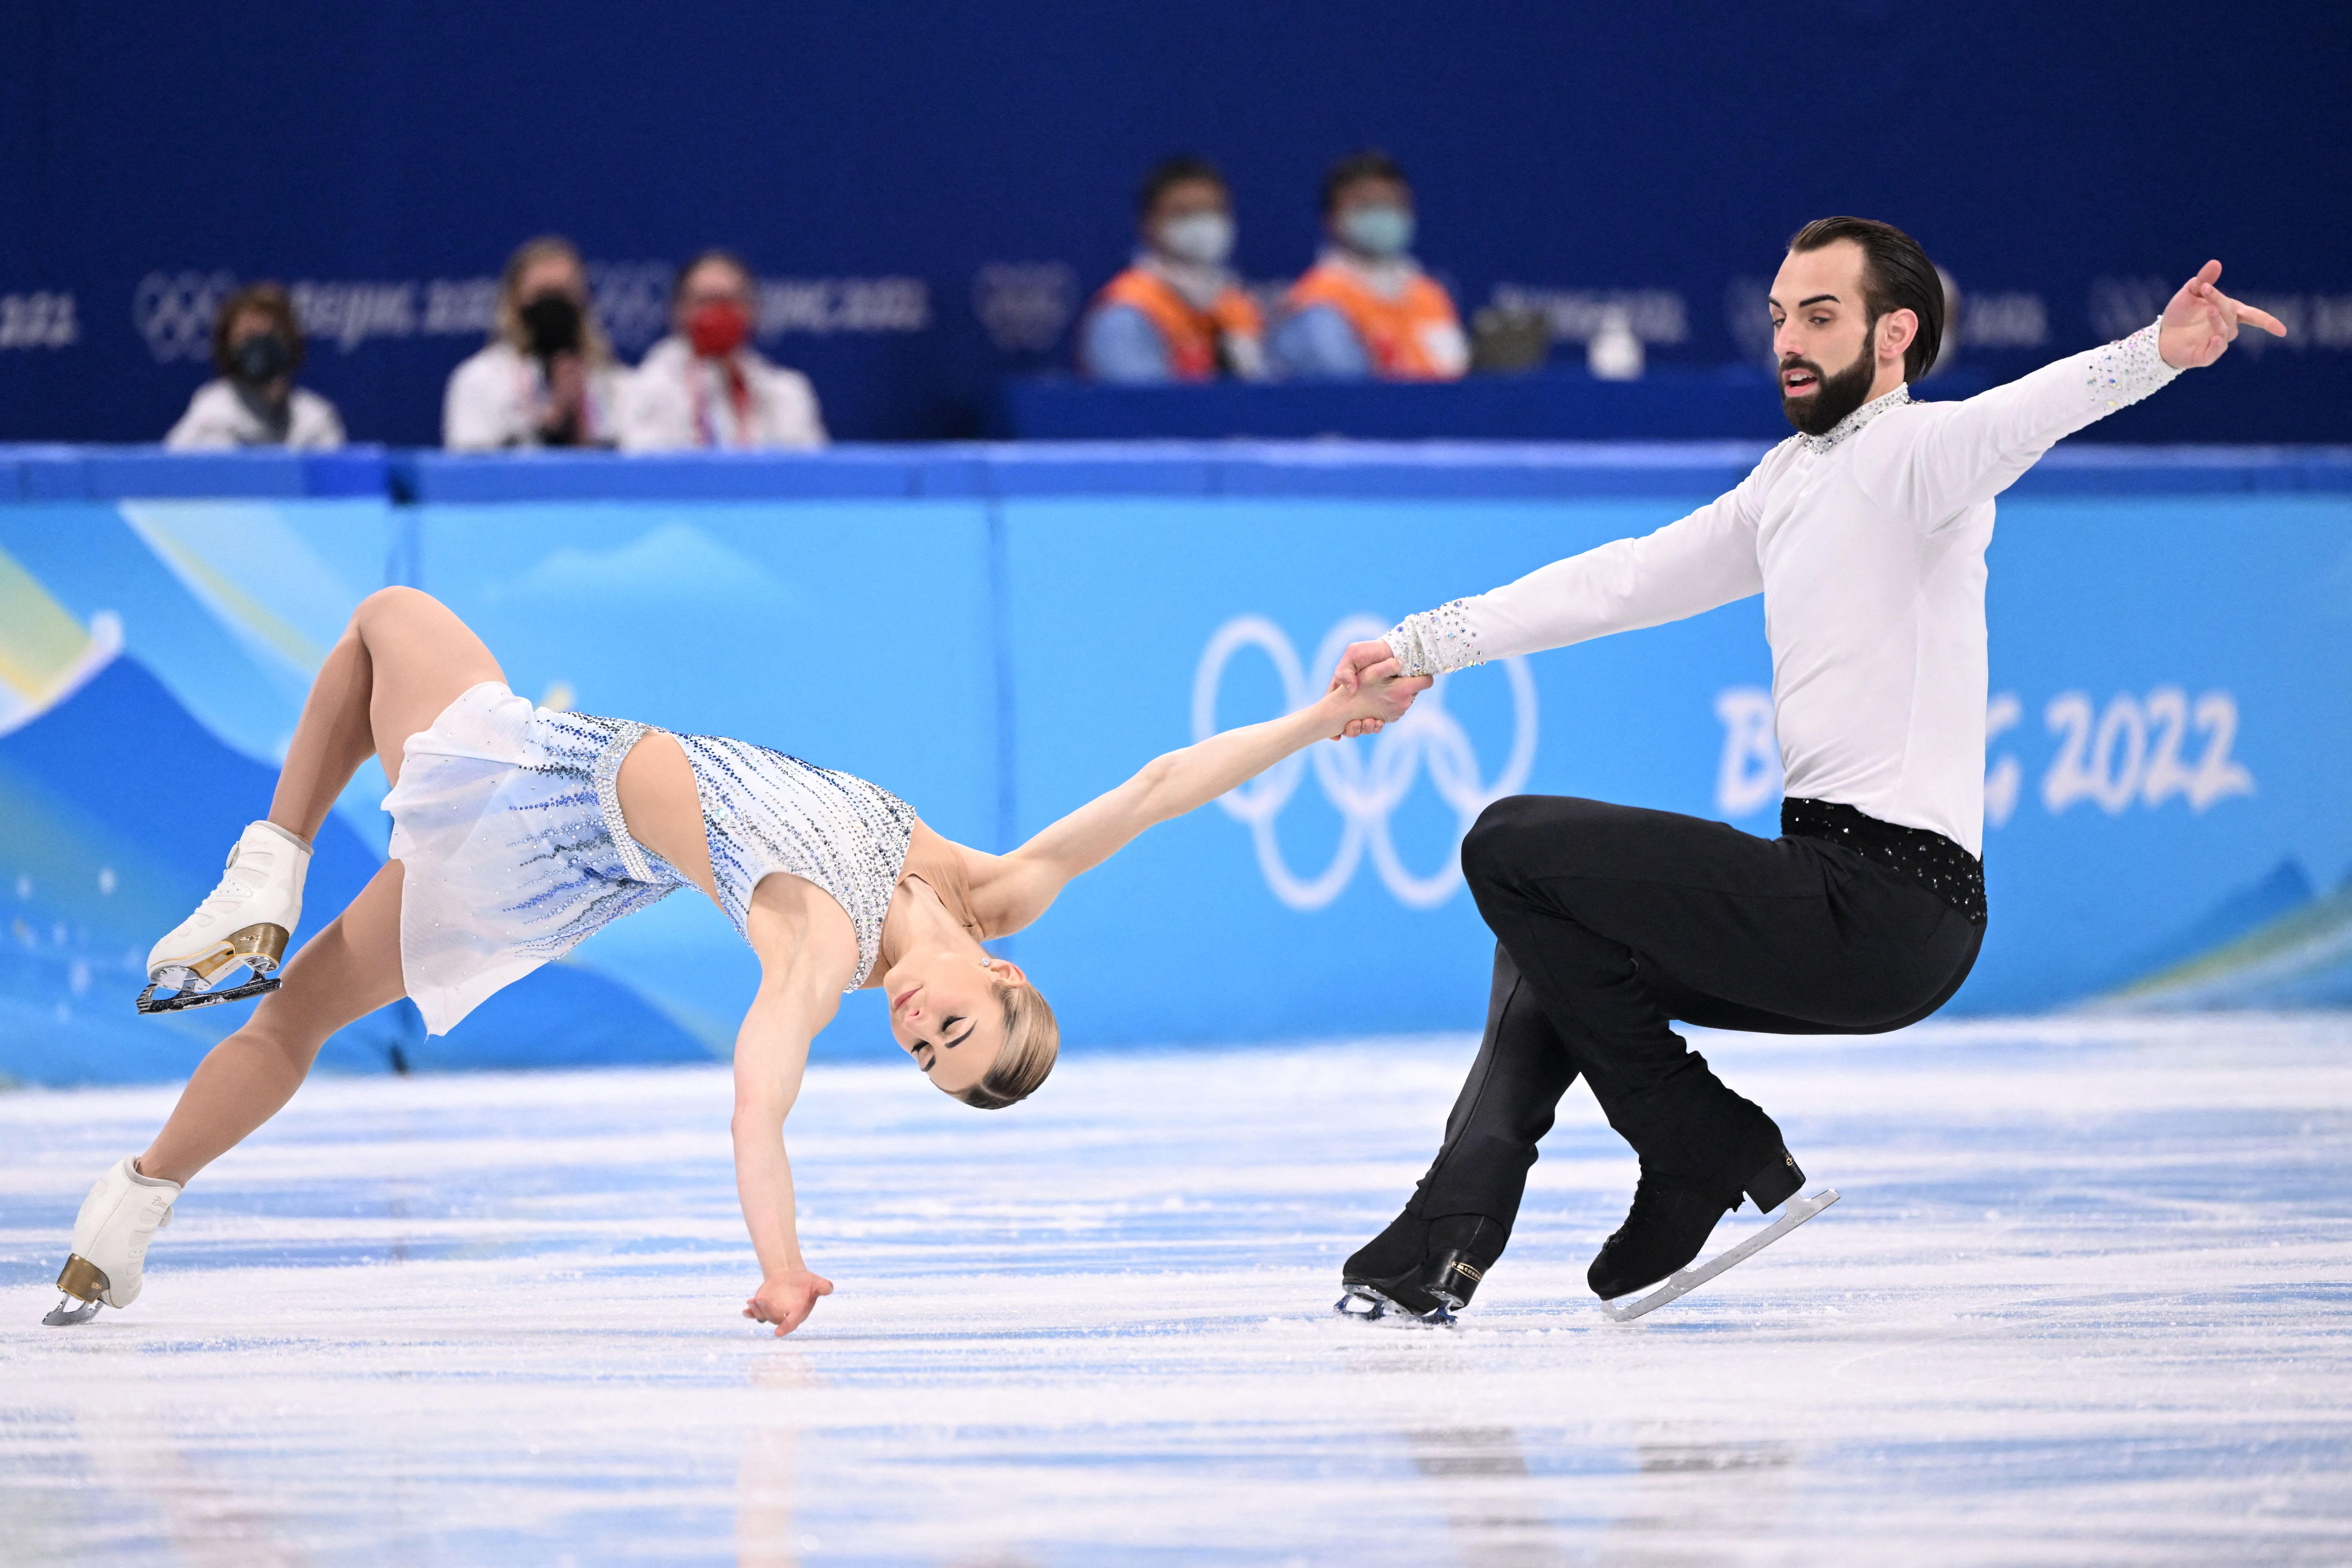
\includegraphics[width=\linewidth]{Ressources/patin.jpg}
        \end{center}
    \end{documentboxenv}
    \end{minipage}
    \begin{minipage}{.49\linewidth}
        \begin{documentboxenv}{Enregistrement d'un mouvement circulaire uniforme}
        \label{doc2}
        \begin{center}
            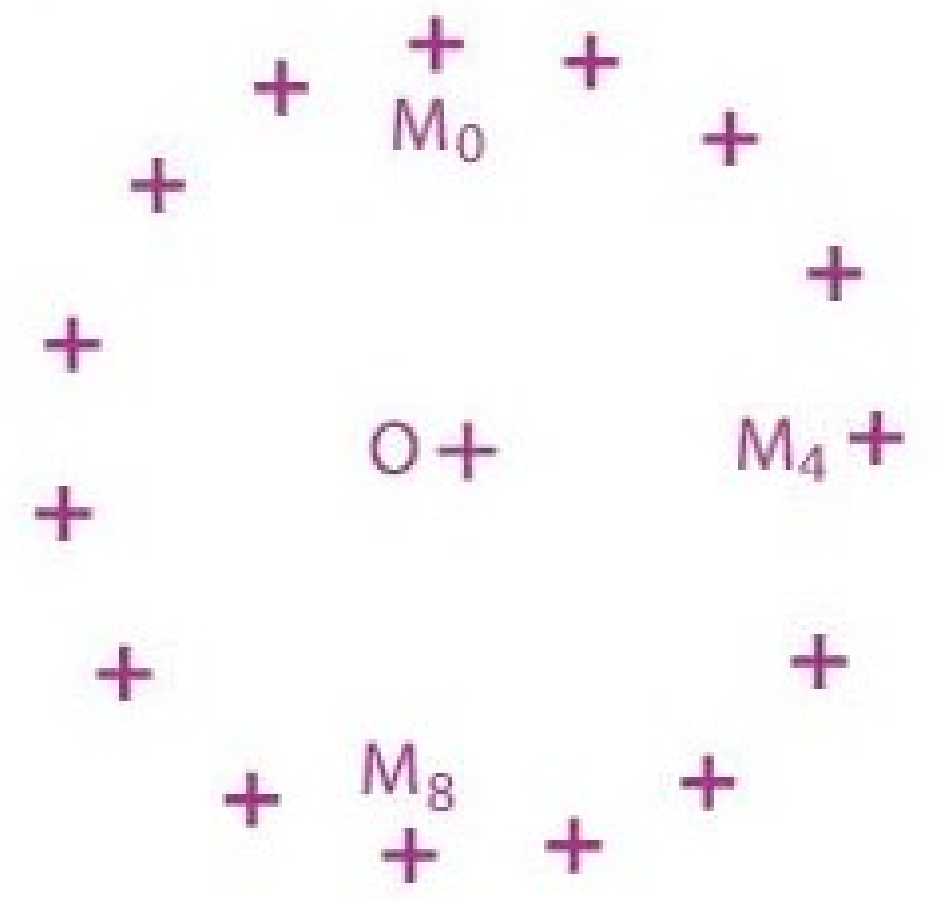
\includegraphics[width=\linewidth]{Ressources/Position_patineuse.png}
        \end{center}
        La patineuse est assomilée à un point matériel. Ses positions successives sont données à l'intervalle de temps $\tau = \SI{40}{\milli\second}$.
        \end{documentboxenv}
    \end{minipage}

    \begin{question}
        \begin{enumerate}
            \item Préciser à l'aide du Doc.~\ref{doc1}, la caractéristique du vecteur vitesse du système \{patineuse\} qui change au cours du mouvement.
            \item Représenter sur le Doc.~\ref{doc2}, les vecteurs vitesses $\vv{v_1}$, $\vv{v_2}$, $\vv{v_9}$ et $\vv{v_{10}}$.
            \item Représenter le vecteur variation de vitesse $\Delta \vv{v_2} = \vv{v_2} - \vv{v_1}$ au point $M_2$. Tracer de même $\Delta vv{v_{10}}$ au moint $M_{10}$. Vérifier que chaque vecteur $\Delta \vv{v}$ a pour direction le rayon du cercle et est orienté vers le centre du cercle, quelle que soit la date $t$.
            \item Montrer que la somme des forces appliquées à la \{patineuse\} est égale à la force exercée sur elle par le patineur : $\sum \vv{Forces} = \vv{F}$.
            \item Comparer les directions et les sens des vecteurs $\vv{F}$ et $\Delta \vv{v}$.
            \item Indiquer les caractéristiques du vecteur $\Delta \vv{v}$ dans le cas où les forces exercées ne se compensent pas, $\sum \vv{Forces} \neq \vv{0}$.
        \end{enumerate}
    \end{question}
\end{document}